% simple cycle
% Author : Jerome Tremblay
\documentclass{standalone}
\usepackage{amsfonts,graphicx,amsmath,amssymb,hyperref,color}
\usepackage[english]{babel}
\makeindex
\frenchspacing
\sloppy
\usepackage{times}
\usepackage{tikz}
\usetikzlibrary{arrows,automata}
\begin{document}
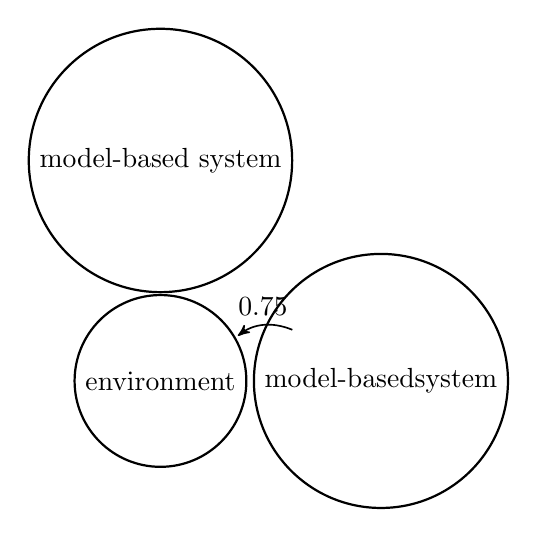
\begin{tikzpicture}[->,>=stealth',shorten >=1pt,auto,node distance=2.8cm,semithick]
\tikzstyle{every state}=[fill=white,draw=black,thick,text=black,scale=1]
\node[state]         (A)              {environment};
\node[state]         (B) [right of=A] {real experience};
\node[state]         (C) [right of=A] {model-based\\ system};
\node[state]         (D) [above of=A] {model-based system};
\path (B) edge  [bend right] node[above] { 0.75} (A);
\end{tikzpicture}
\end{document}
